\subsection{UC9 - Mostra applicazione}
\begin{figure}[H]
    \centering
    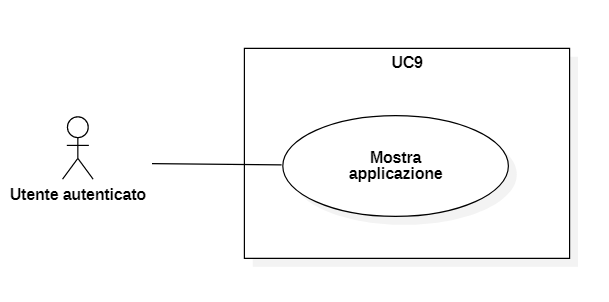
\includegraphics[scale = 0.7]{components/img/UC9.png}
    \caption{UC9 - Mostra applicazione}
\end{figure}
\begin{itemize}
\item \textbf{Attore Primario:} Utente autenticato;
\item \textbf{Precondizione:} L'applicazione si trova nell'area di notifica;
\item \textbf{Postcondizione:} L'applicazione viene mostrata a tutto schermo;
\item \textbf{Scenario principale:}
    \begin{enumerate}
    \item L'utente visualizza l'area di notifica;
    \item L'utente clicca sull'icona dell'applicazione.
    \end{enumerate}
\end{itemize}